\documentclass[a4paper, 12pt]{article}
\usepackage{amsmath, amssymb, amsthm}
\usepackage{geometry}
\usepackage{tcolorbox}
\geometry{hmargin=2.5cm, vmargin=2.5cm}

\renewcommand*{\today}{03 octobre 2024}

\title{Analyse | CM: 5}
\author{Par Lorenzo}
\date{\today}

\newtheorem{theorem}{Théorème}[section]
\newtheorem{definition}{Définition}[section]
\newtheorem{example}{Example}[section]
\newtheorem{remark}{Remarques}[section]
\newtheorem{lemme}{Lemme}[section]

\newtheorem{_proposition}{Proposition}[section]
\newenvironment{proposition}[1][]{
    \begin{_proposition}[#1]~\par
    \vspace*{0.5em}
}{%
    \end{_proposition}%
}

\newenvironment{rdem}[1][]{
    \begin{tcolorbox}[colframe=black, colback=white!10, sharp corners]
        #1
}{%
    \end{tcolorbox}
     
}

\newtheorem{_demonstration}{Démonstration}[section]
\newenvironment{demonstration}[1][]{
    \begin{_demonstration}[#1]~\par
    \vspace*{0.5em}
}{%
    \end{_demonstration}%
    \qed%
}

\newtheorem*{_demonstration*}{Démonstration}
\newenvironment{demonstration*}[1][]{
    \begin{_demonstration*}[#1]~\par
    \vspace*{0.5em}
}{%
    \end{_demonstration*}%
    \qed%
}

\newenvironment{proprietes}{
    \noindent\textbf{Propriétés}
    \begin{enumerate}
}{
    \end{enumerate}
}

\newenvironment{ldefinition}{
    \begin{definition}~\par
    \vspace*{0.5em}
    \begin{enumerate}
}{
        \end{enumerate}
        \end{definition}
}

\newenvironment{lexample}{
    \begin{example}~\par
    \vspace*{0.5em}
    \begin{enumerate}
}{
        \end{enumerate}
        \end{example}
}

\newtheorem{_methode}{Méthode}[section]
\newenvironment{methode}{
    \begin{_methode}~\par
    \vspace*{0.5em}
}{
        \end{_methode}
}

\def\N{\mathbb{N}}
\def\Z{\mathbb{Z}}
\def\Q{\mathbb{Q}}
\def\R{\mathbb{R}}
\def\C{\mathbb{C}}
\def\K{\mathbb{K}}

\def\un{(u_n)_{n \in \N}}
\def\xn#1{(#1_n)_{n \in \N}}

\def\o{\overline}
\def\eps{\varepsilon}

\newcommand{\lt}{\ensuremath <}
\newcommand{\gt}{\ensuremath >}

\begin{document}

\maketitle

\begin{example}
    \item $\bullet$ $(n)_{n \in \N}$ est la suite des entiers.
    \item $\bullet$ $((-1)^n)_{n \in \N}$ est la suite alternant entre 1 et -1.
    \item $\bullet$ $(F_n)_{n \in \N}$ définie par $F_0=1, F_1=1, F_{n+2}=F_{n+1}+F_n$
    est la suite de Fibonacci.
\end{example}

\begin{remark}
    Ne pas confondre la fonction avec une suite ($(\sqrt{n})_{n \in \N}$ différent de $f(x)= \sqrt{x}$)
\end{remark}

\subsubsection{Suites majorées, minorées, bornées}

\begin{definition}
    Soit $\un$ une suite de nombre réels.
    
    \item On dit que la suite $\un$ est
    \textbf{majorée} si $\exists M \in \R, \forall n \in \N, u_n \leq M$.
    
    \item On dit que la suite $\un$ est
    \textbf{minorée} si $\exists M \in \R, \forall n \in \N, M \leq u_n$.

    \item On dit que la suite $\un$ est
    \textbf{bornée} si la suite $\un$ est majorée et minorée.\par
    (i.e. $\exists M \in \R, \forall n \in \N, |u_n| \leq M$)
\end{definition}

\begin{definition}
    \item La suite $\un$ est \textbf{croissante} si $\forall n \in \N, u_{n+1} \geq  u_n$.
    
    \item La suite $\un$ est \textbf{strictement croissante} si $\forall n \in \N, u_{n+1} \gt  u_n$.
    
    \item La suite $\un$ est \textbf{décroissante} si $\forall n \in \N, u_{n+1} \leq  u_n$.

    \item La suite $\un$ est \textbf{strictement décroissante} si $\forall n \in \N, u_{n+1} \lt  u_n$.

    \item On dit que la suite est \textbf{monotone} si elle est croissante ou décroissante.
\end{definition}

\begin{remark}
    Pour vérifier la monotonie d'une suite:

    \item Soit $u_{n+1} - u_n \geq 0 \implies$ croissante
    \item Soit on calcule (avec $u_n \neq 0$) $\dfrac{u_{n+1}}{u_n} \geq 1 \implies$ croissante

    On préfère la première pour les suites arithmétiques et la deuxième pour les suites géométriques.
\end{remark}

\subsection{Limites}

\subsubsection{Limit finie, limite infinie}

\begin{definition}
    La suite $\un$ admet pour limite $l \in \R$ si
    $$
    \forall \varepsilon \gt 0, \exists N \in \N, \forall n \geq N, |u_n - l| \leq \varepsilon
    $$

    On dit que la suite $\un$ tend vers l quand n tend vers l'infini, ou
    $$
    \lim_{n \to \infty} u_n = l
    $$
\end{definition}

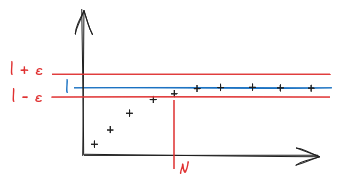
\includegraphics{img/limite.png}

\begin{remark}
    On utilise $\varepsilon$ pour parler d'un nombre très petit.
\end{remark}

\begin{definition}
    La suite $\un$ tend vers $+\infty$ si elle devient aussi grande que l'on souhaite quand n
    devient grand, autrement dit

    $$
    \forall A \gt 0, \exists N \in \N, \forall n \geq N, u_n \geq A
    $$

    La suite $\un$ tend vers $-\infty$ si elle devient aussi petite que l'on souhaite quand n
    devient grand, autrement dit

    $$
    \forall A \gt 0, \exists N \in \N, \forall n \geq N, u_n \leq -A
    $$
\end{definition}

\begin{definition}
    \item $\un$ \textbf{converge} si elle admet une limite finie.

    \item $\un$ \textbf{diverge} si elle admet l'infini comme limite ou si elle n'a pas de limite.
\end{definition}

\begin{proposition}
    Si une suite converge, alors sa limite est unique.
\end{proposition}

\begin{demonstration}
    Soit $\un$ une suite qui admet deux limite, $l_1 \neq l_2$.
    
    $$
    \lim_{n \to +\infty}u_n = l_1 \implies
    \forall \varepsilon_1, \exists N_1 \in \N, \forall n \geq N_1, |u_n - l_1| \leq \varepsilon_1
    $$
    
    $$
    \lim_{n \to +\infty}u_n = l_2 \implies
    \forall \varepsilon_2, \exists N_2 \in \N, \forall n \geq N_2, |u_n - l_2| \leq \varepsilon_2
    $$

    Pour $\varepsilon_1 = \varepsilon = \varepsilon_2 \gt 0$
    
    $\exists N = max(N_1, N_2), \forall n \geq \N, |u_n - l_1| \lt \varepsilon \text{ et } |u_n - l_2| \lt \varepsilon$

    Donc $|l_1 - l_2| = |l_1 - u_n + u_n - l_2| = |(l_1 - u_n) + (u_n - l_2)| \leq |l_1 - u_n| + |u_n - l_2| \lt \varepsilon + \varepsilon = 2 \varepsilon$

    Il suffit de prendre $\varepsilon \lt \dfrac{|l_1 - l_2|}{2}$, ainsi

    $$
    |l_1 - l_2| \lt 2\varepsilon \leq |l_1 - l_2|
    $$

    \begin{rdem}
        Ce qui est absurde, Finalement $l_1 = l_2$
    \end{rdem}
\end{demonstration}

\subsubsection{Propriétés des limites}

\begin{proprietes}
    \item $\lim_{n \to +\infty} u_n = l \iff \lim_{n \to +\infty}(u_n - l) = 0 \iff \lim_{n \to +\infty} |u_n - l| = 0$
    \item $\lim_{n \to +\infty} u_n = l \implies \lim_{n \to +\infty}|u_n| = |l|$
\end{proprietes}

\begin{remark}
    C'est en général faux dans l'autre sens. Par exemple pour $u_n = (-1)^n$,
    $|u_n|=1$ donc $\lim_{n \to \infty} |u_n| = 1$ mais $\un$ n'a pas de limite (-1, 1, -1, 1, ...).
\end{remark}

\begin{proposition}
    Soient $\un$ et $\xn{v}$ deux suites convergentes.

    \item
    $$
    \lim_{n \to +\infty} u_n = l \implies \forall \delta \in \R, \lim_{n \to +\infty}(\delta u_n) = \delta l
    $$
    
    \item
    $$
    \lim_{n \to +\infty} u_n = l \text{ et } \lim_{n \to +\infty} v_n = l' \implies \lim_{n \to +\infty}(u_n + v_n) = l + l' \text{ et } \lim_{n \to +\infty}(u_n \times v_n) = l \times l'
    $$
    
    \item
    $$
    \exists N \in \N, \forall n \in \N, n \geq N, l \neq 0 \text{ et } u_n \neq 0 \implies \lim_{n \to +\infty} \dfrac{1}{u_n}=\dfrac{1}{l}
    $$
\end{proposition}

\begin{demonstration}

    \begin{align*}
        \lim_{n \to +\infty} u_n = l &\implies \forall \varepsilon \gt 0, \exists N \in \N, n \geq N, |u_n - l| \leq \varepsilon \\
        &\implies \forall \varepsilon \gt 0, \exists N \in \N, n \geq N, |\delta|| u_n - l|  \leq |\delta|\varepsilon \\
        &\implies \forall \varepsilon' \gt 0, \exists N \in \N, n \geq N, |\delta u_n - \delta l|  \leq |\delta|\varepsilon = \varepsilon' \\
        &\implies \lim_{n \to +\infty} \delta u_n = \delta l 
    \end{align*}

    \begin{align*}
        \lim_{n \to +\infty} u_n = l \implies \forall \varepsilon \gt 0, \exists N \in \N, n \geq N, |u_n - l| \leq \varepsilon \\
        \lim_{n \to +\infty} v_n = l' \implies \forall \varepsilon \gt 0, \exists N \in \N, n \geq N, |v_n - l'| \leq \varepsilon \\
        |u_n - l| + |v_n - l'| \geq |u_n - l + v_n - l'| = |(u_n + v_n) - (l + l')| \\
        \implies |(u_n + v_n) - (l + l')| \leq 2 \varepsilon = \varepsilon'
    \end{align*}

    \color{red}
    À compléter
    \color{black}
    \begin{align*}
        \lim_{n \to +\infty} u_n &= l \implies \forall \varepsilon \gt 0, \exists N \in \N, n \geq N, |u_n - l| \leq \varepsilon \\
        \lim_{n \to +\infty} v_n &= l' \implies \forall \varepsilon \gt 0, \exists N \in \N, n \geq N, |v_n - l'| \leq \varepsilon \\
        |u_n \times v_n - l \times l'| &= |u_n \times v_n - l \times v_n + l \times v_n - l \times l'| \\
        &= |v_n (u_n - l) + l (v_n - l')| \\
        &\leq |v_n (u_n - l)| + |l (v_n - l')| \\
        &= |v_n| |u_n - l| + |l| |v_n - l'|\\
    \end{align*}

    \color{red}
    À faire
    \color{black}
    \begin{align*}
        \lim_{n \to +\infty} u_n = l &\implies \forall \varepsilon \gt 0, \exists N \in \N, n \geq N, |u_n - l| \leq \varepsilon \\
    \end{align*}

\end{demonstration}

\end{document}
